\chapter{Tools installation}

\section{Acquia Dev Desktop}

The Acquia Dev Desktop provides an easy way to run a Drupal site on your local computer. The tool includes an AMP (Apache, MySql, PHP) stack which allows your Drupal application to be executed. You can use it to create a new Drupal site and manage it.

\subsection{Installation}

\begin{itemize}
	\item Download the version of Acquia dev desktop for your operating system at \url{https://www.acquia.com/downloads}.
	\item When your download is complete, run the installer.
	\item Keep clicking Next, accept the licence agreement and select the installation location for dev desktop as well as the location where your Drupal sites will be stored. In this course we use the \url{C:\drupal_sites} directory but you can change this to a directory of your preference. It is advised to choose a directory that is short and has no spaces.
	
	\begin{figure}[H]
		\centering
		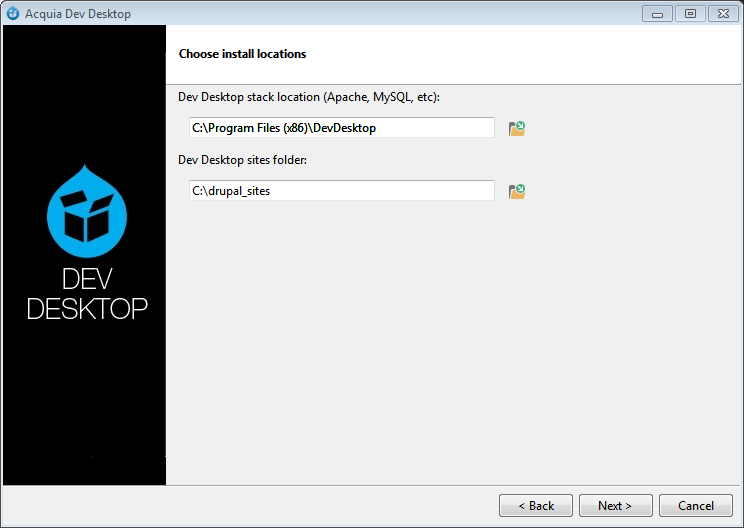
\includegraphics[width=\textwidth]{chapter2/dev_desktop_install_site_location}
		\caption{Installation location}
		\label{fig:dev_desktop_install_site_location}
	\end{figure}
	
	\item When the installer is complete you are ready to create your first site. Before we do that we'll install some useful tools that will help us during development.
	
	
\end{itemize}

\section{NetBeans}

When we are developing our Drupal site we'll write PHP, html and css code. In this course we use the Netbeans ide to do all this. You can download the NetBeans editor at: \url{https://netbeans.org/downloads/}. You can choose to download the version for HTML5 an PHP or the ALL version.

\subsection{installation}

Run the NetBeans installer. You can use the default settings or change them to your liking. 

\subsection{configuration}

Next we'll configure NetBeans to associate the Drupal file extensions to the correct file types. For example \textbf{.module} files should be opened as a PHP file.
Go to \textbf{Tools \textgreater Preferences \textgreater Miscellaneaus \textgreater Files} there you can add new file extensions and associate the file type. Associate the following extensions with the \textbf{text/x-php5} MIME type:

\begin{itemize}
	\item module
	\item install
	\item test
	\item profile
	\item theme
	\item engine
\end{itemize}

Associate the following extensions with the \textbf{text/plain} MIME type:
\begin{itemize}
	\item info
	\item po
\end{itemize}

\begin{figure}[H]
	\centering
	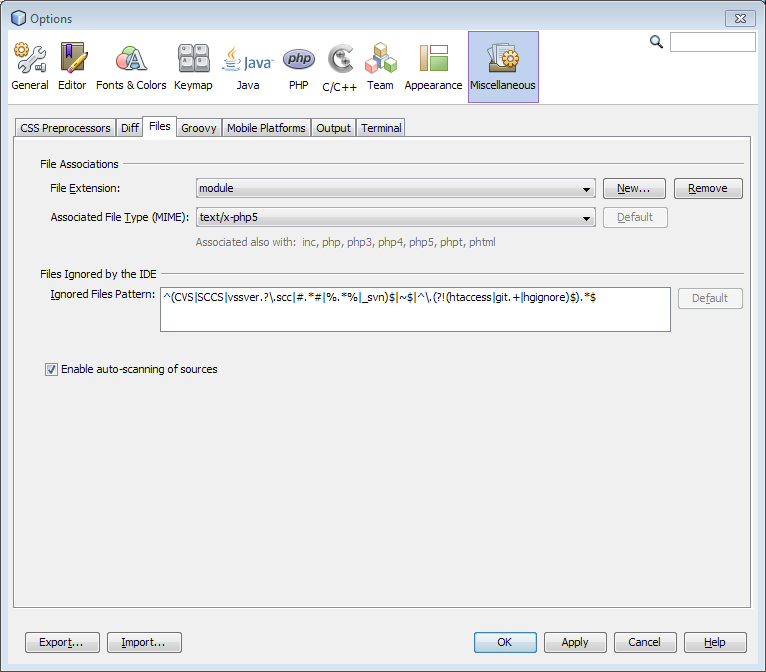
\includegraphics[width=\textwidth]{chapter2/file_extensions_configuration}
	\caption{Extension configuration}
	\label{fig:file_extension_configuration}
\end{figure}

\section{WinLess}

WinLess is a less compiler for windows. The less language makes it easier to write css code. In this course we assume you are familiar with css and less so we won't go into depth on how to write less code. To install the less compiler, download the latest version of WinLess from \url{http://winless.org/} and run the installer. 

WinLess allows you to select a less file and automatically compile it to a css file in the directory you specify. (see Figure: \ref{fig:winless_interface})

	\begin{figure}[H]
		\centering
		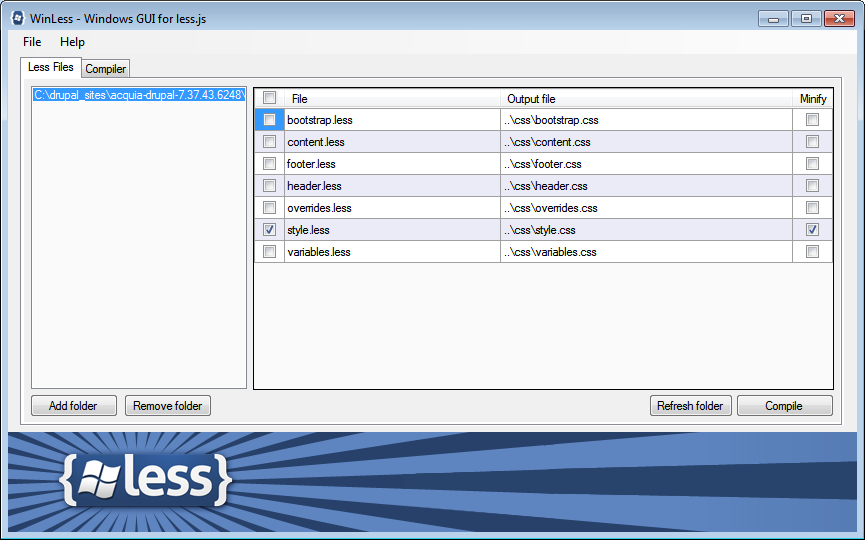
\includegraphics[width=\textwidth]{chapter2/winless_interface}
		\caption{WinLess interface}
		\label{fig:winless_interface}
	\end{figure}
	
\section{Drush}

Drush is a command line tool which makes it easy to manage your site. Since Drush is included in the Acquia dev desktop installation you don't need to install it separately. You can test your Drush installation by opening a command line window and typing \textbf{drush} and hitting enter.

\section{GIT} 

GIT is a versioning system, it enables you to share and manage your code. You can download the git installer here: \url{https://git-scm.com/downloads}

\subsection{Installation}

\begin{itemize}
	\item Run the installer. 
	\item In the window \textbf{Adjusting your PATH environment} select the option \textbf{Use Git from the Windows Command Prompt}
	\item In the next window select \textbf{UseOpenSSH}
	\item Configure the line endings as \textbf{Checkout Windows-style, commit Unix-style line endings}
	\item Finish the installer wizard.
\end{itemize}
 